\subsection{Non-linear sloshing in a rectangular container}%Ansari

Free surface oscillations of a liquid confined in a closed container (sloshing phenomenon) are an important issue when big amounts of liquid are industrially transported. The phenomenon involves two fluids that share a free surface boundary separating them, normally the density of the upper fluid is several orders of magnitude less than the bottom one. This phenomenon has proven of great interest due to the fact that violent impacts of the fluid can affect the structural integrity of the container.

For studied cases in this section, the sloshing phenomenon is produced by a horizontal harmonic excitation $x = a_h (\sin \omega_h t)$, where $a_h$ is the excitation amplitude and $\omega_h$ is the excitation frequency of the rectangular tank where the two fluid phases are contained. The tank is divided in two parts, the bottom part is water with a density of $\rho_{I} = 1000 [kg/m^3]$ and the top part contains a fluid with different densities $\rho_{II} = 1.3, 50, 200, 800 [kg/m^3]$, depending on the studied case. The dimensions of the tank are $a$(width) by $b$(height) and the initial free surface is at height $h$ from the bottom of the tank, see Figure \ref{fg:ansari-config}. The free surface starts the simulation as a horizontal line and is subsequently deformed by the tank excitation and the flow dynamics.

\begin{figure}[H]
  \begin{center}
      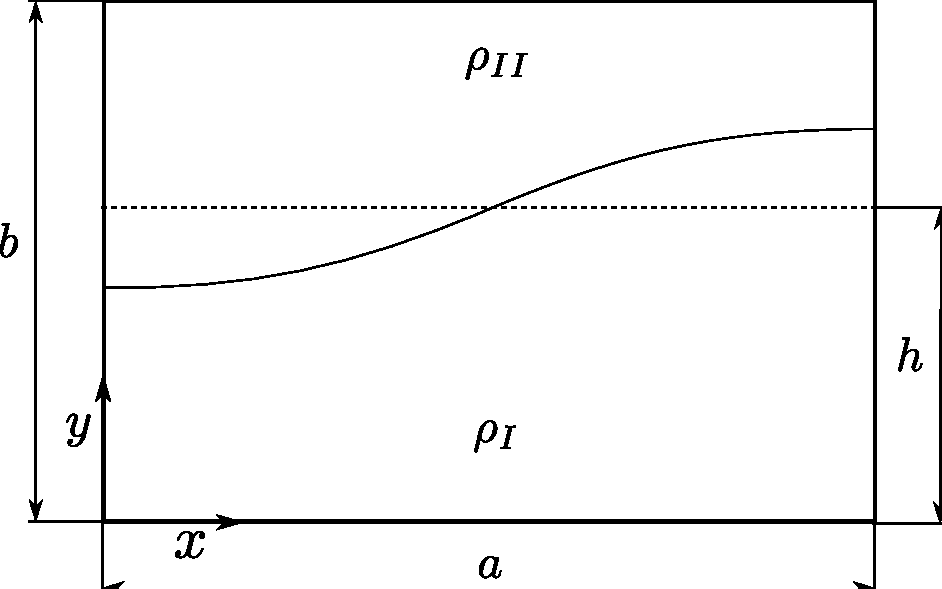
\includegraphics[width=.6\columnwidth]{images/ansari_config.pdf}
  \end{center}
  \caption{\label{fg:ansari-config} Configuration of the Non-linear sloshing in a rectangular container case. Initial condition is represented by dashed lines. Continuous line represents the position of the free-surface for a certain time.}
\end{figure}

For the different cases in this report, a 2D rectangular tank $a=1.0[m]$ width by $b=1.0[m]$ height is used. The initial height of the interface is $h=0.5[m]$ and the lateral excitation applied is $x=0.05\sin(3t)$. The simulations were performed considering the
flow as laminar and non-viscous, hence no turbulence model was used and slip boundary conditions are taken. Density was modified according to the considered ratios $\sigma=\frac{\rho{II}}{\rho{I}}$. A two dimensional Cartesian mesh of $450\times225$, splitted into triangles, has been used in all cases.

Reference results for this case are taken from \cite{Goni13} which uses the codes STARCCM+ and \OF to obtain numerical solutions and reports the free surface displacement on the left wall of the container. Those simulations use the same grid as presented above, but, in order to avoid numerical instabilities, they limit the $CFL$ number to $CFL_{max}=0.5$ then they use $\Delta t \approx 0.001$. In PFEM-2 simulations do not exist that restriction then $\Delta t$ is fixed to $0.01$, reaching $CFL_{max}\approx5$. 
Figure \ref{fg:ansari-results} presents the free surface displacement reported on the left wall of the container for different density ratios. For each one of them, PFEM-2 simulations shows a good agreement with reference solutions, further more considering that the time step used is around ten times bigger than the used in \cite{Goni13}.


  \begin{figure}[h]
  \centering
    \subfloat[]{
	  \label{fg:ansari-1}         %% Etiqueta para la primera subfigura
	  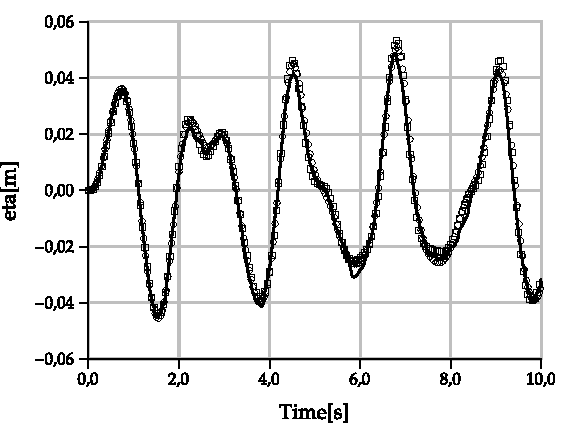
\includegraphics[width=.49\columnwidth]{images/ansari_1.pdf}
    }
    %%----segunda subfigura----
    \subfloat[]{
	  \label{fg:ansari-2}         %% Etiqueta para la segunda subfigura
	  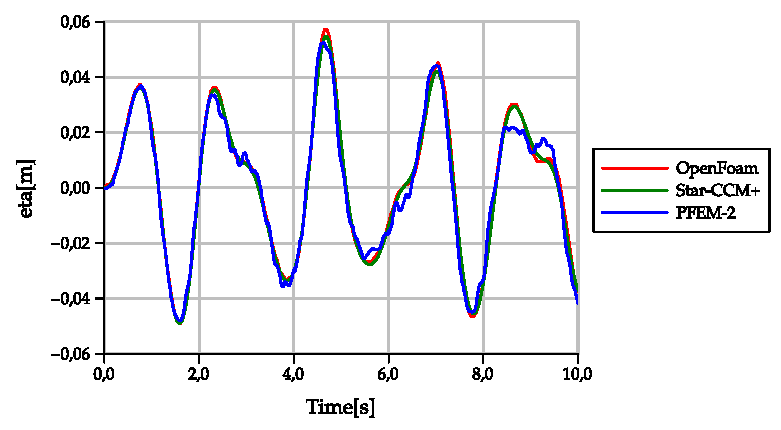
\includegraphics[width=.49\columnwidth]{images/ansari_2.pdf}
    } \\
    \subfloat[]{
	  \label{fg:ansari-3}         %% Etiqueta para la primera subfigura
	  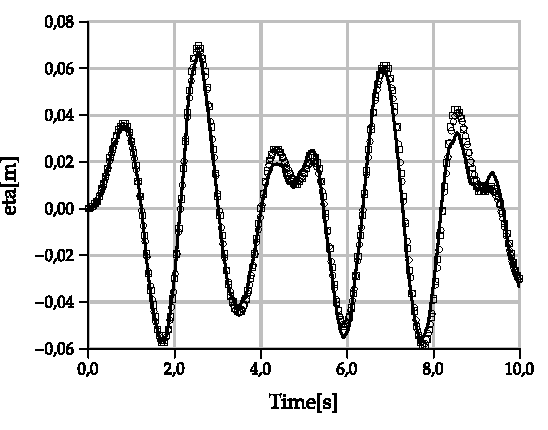
\includegraphics[width=.49\columnwidth]{images/ansari_3.pdf}
    }
    %%----segunda subfigura----
    \subfloat[]{
	  \label{fg:ansari-4}         %% Etiqueta para la segunda subfigura
	  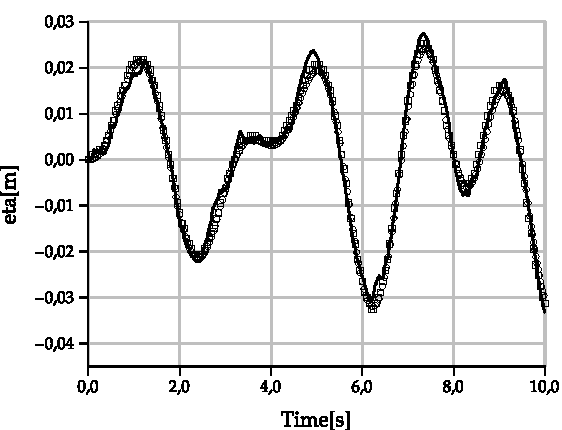
\includegraphics[width=.49\columnwidth]{images/ansari_4.pdf}
    }
   \caption{Level of height on the left wall for a two phase flow for different density ratios. Figure \ref{fg:ansari-1}: $\sigma=0.0013$, Figure \ref{fg:ansari-2}: $\sigma=0.05$, Figure \ref{fg:ansari-3}: $\sigma=0.2$ and Figure \ref{fg:ansari-4}: $\sigma=0.8$. References:\ \Circle \ STARCCM, \Square \ OpenFOAM and filled line PFEM-2.}
   \label{fg:ansari-results}                %% Etiqueta para la figura entera
\end{figure}

\subsubsection{Enrichment and density ratio issues}

The PFEM-2 results presented in the previous section were using the continuous enrichment strategy, which allows to use the same formulation independently of the Froude Number of the problem. However, as it was mentioned before, without ensuring continuity between elements when the enriched shape functions are used, the assumption that the inter-elemental boundary terms from the weakening of the Poisson equation might be avoided is not true. In this subsection, problems that appear using large Froude numbers (which represent the relation between the inertial and gravitational forces and is defined by $Fr = \dfrac{U^2}{gL}\dfrac{\rho_I}{\rho_I-\rho_{II}}$) are shown. This behavior is also commented, but not reported, by Coppola\cite{Coppola05}. 

The Figure \ref{fg:ansari-results-b} shows a comparison between the level of the height calculated by PFEM-2 using continuous enrichment, discontinuous enrichment and no-enrichment in the extreme density ratio cases. It must be mentioned that the results were obtained with the enrichment shape functions presented in \ref{eq:enrich-1a}, however using \ref{eq:enrich-2a} similar conclusions were reached.

Low density ratio generates higher $Fr$ values, as happens in the case $\sigma=0.8$ of the sloshing case, and in the Figure \ref{ansari-4b} a comparison between different PFEM-2 results is presented. Without using any strategy of enrichment, the solution might be not noisy due to the low density ratio, but from the height levels it can be viewed that the typical mass-loss appears deteriorating the overall solution. With discontinuous enrichment (it is, condensing the equation system \ref{eqsys-poisson}) the solution is too smooth. We concluded that the diffusive behavior with discontinuous enrichment appears because of avoiding the inter-elemental boundary terms from the weakening the right hand side of \ref{poisson}. This idea is confirmed when discontinuous enrichment is used but without weakening the divergence of the velocity and a solution very similar to continuous enrichment is obtained. Not integrating by parts the divergence term requires imposing a pressure gradient on boundaries: with low density ratios we can impose the previous gradient value $\nabla p^n$ on boundaries, but this approximation is not valid when there is a gravitational field, large density ratio, and the fluid is not at rest.

On the other hand, in the Figure \ref{fg:ansari-1b} the case $\sigma=0.0013$ is presented. The graphic shows that the solution obtained with continuous enrichment is almost equal to the discontinuous enrichment solution. The results without enrichment are noisy, showing the problem with spurious velocity that appears in the free surface if no improvements in this region are done.

  \begin{figure}[h]
  \centering
    \subfloat[]{
	  \label{fg:ansari-1b}         %% Etiqueta para la primera subfigura
	  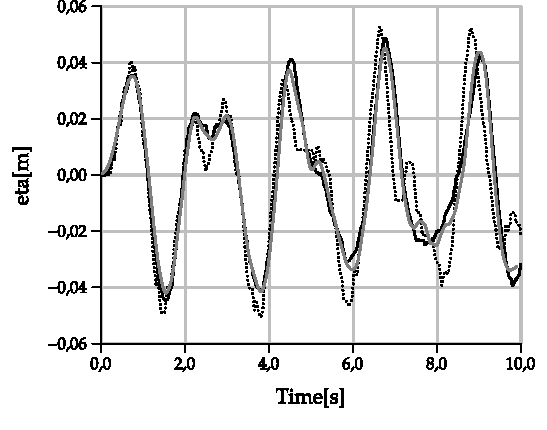
\includegraphics[width=.49\columnwidth]{images/ansari_1b.pdf}
    }
    %%----segunda subfigura----
    \subfloat[]{
	  \label{fg:ansari-4b}         %% Etiqueta para la segunda subfigura
	  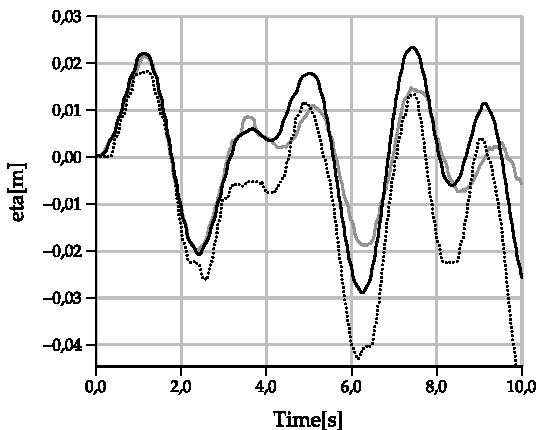
\includegraphics[width=.49\columnwidth]{images/ansari_4b.pdf}
    }
   \caption{Level of height on the left wall for a two phase flow for different density ratios. Figure \ref{fg:ansari-1b}: $\sigma=0.0013$ and Figure \ref{fg:ansari-4b}: $\sigma=0.8$. References: filled black line continuous enrichment, filled gray line discontinuous enrichment, and dotted line without enrichment.}
   \label{fg:ansari-results-b}                %% Etiqueta para la figura entera
\end{figure}

In the current implementation choosing continuous enrichment increases in a $50\%$ the total CPU times comparing with discontinuous ones, but the former formulation can be applied on a wide range of situations. With discontinuous enrichment, better computing times can be obtained, but the formulation is not general now: to integrate by parts or not the term with velocity divergence will depend on principally the density ratio of the problem to solve.

\clearpage
